\documentclass[a4paper,conference]{IEEEtran}

\usepackage{amsmath}
\usepackage{graphicx}
\usepackage{cite}
\usepackage{stfloats}
\usepackage{algorithm}
\usepackage{algpseudocode}
\usepackage{bm}

\begin{document}

\title{Genetic Painting}
\author{\IEEEauthorblockN{Liangwang Ruan}
  \IEEEauthorblockA{Peking University\\
  Email: ruanliangwang@pku.edu.cn\\
  Student ID: 2101111577}}
\maketitle



\begin{abstract}
  The paper proposes a genetic algorithm to let the computer learn how to draw like human. Given a reference image, the algorithm can generate a sequence of geometry primitives to mimic the strokes on the canvas. User can control the level of details of the painted image by adjusting the stroke size limit and stroke number. 
\end{abstract}
\section{Introduction}
Generative art refers to art that in whole or in part has been created with the use of an autonomous system, has been widely studied over the past decades. A specific branch of generative art uses computer algorithms to show(most visually) regularity of mathematical patterns and show variability from pseudo-random numbers, it's known as algorithmic art. A typical example of algorithmic art is fractal art generated by iteration algorithms in complex domain as shown in Fig. \ref{fig:fracal}.
\begin{figure}[htp]
  \centering
  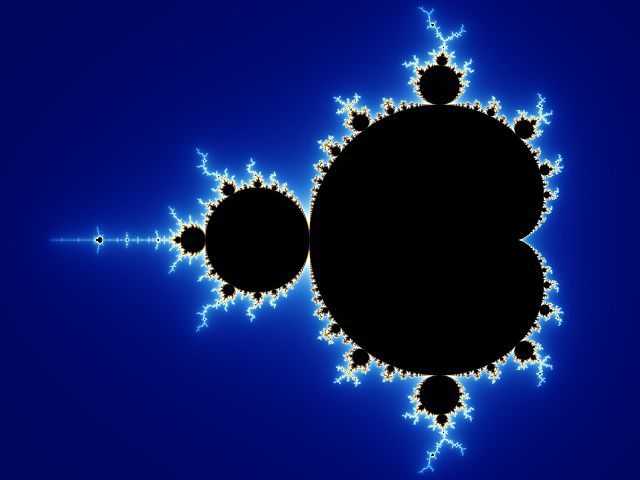
\includegraphics[width=.8\columnwidth]{imgs/mandelbrot_set.jpg}
  \caption{Mandelbrot Set \copyright From Wikipedia}
  \label{fig:fracal}
\end{figure}

Intelligent optimization algorithms are especially designed to deal with NP-hard, non-convex, non-smooth optimization problems, include genetic algorithms, simulated annealing algorithms, ant colony algorithms, etc. Many of them are inspired from biological and natural behaviors, like the genetic algorithms are simulating the evolution theory of Darwin, the ant colony algorithms are imitating the foraging behavior of the ants. The complexity of the problem itself and the bionics nature of these methods make them can generate complex, fascinating visual arts. Examples include 3D animation\cite{e22111284}, 2D drawing\cite{ant-colony}, image triangulation\cite{triangula}. This paper is one of these works, trying to use the genetic algorithm to let the computer learn how to draw like human. To be more specific, the algorithm learns to draw one stroke of paint at a time, at last get a similar painting work like the given image. This work is \textbf{not} the first work to do this task, many other artists have tried the same task with other intelligent optimization algorithms\cite{ant-colony}\cite{primitive}\cite{geometrize}, but this work is the first to apply genetic algorithms to this task.
\begin{figure*}[ht]
  \centering
  
\includegraphics[width=.18\textwidth]{imgs/seagull/sampling_mask20.png}
  
\includegraphics[width=.18\textwidth]{imgs/seagull/sampling_mask40.png}
  
\includegraphics[width=.18\textwidth]{imgs/seagull/sampling_mask60.png}
  
\includegraphics[width=.18\textwidth]{imgs/seagull/sampling_mask80.png}
  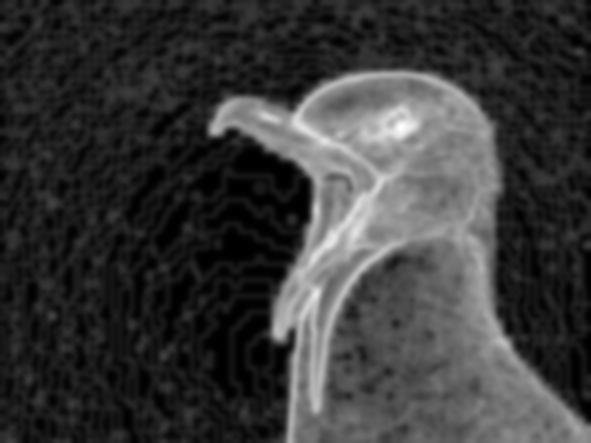
\includegraphics[width=.18\textwidth]{imgs/seagull/sampling_mask99.png}\\
  \vspace{0.1cm}
  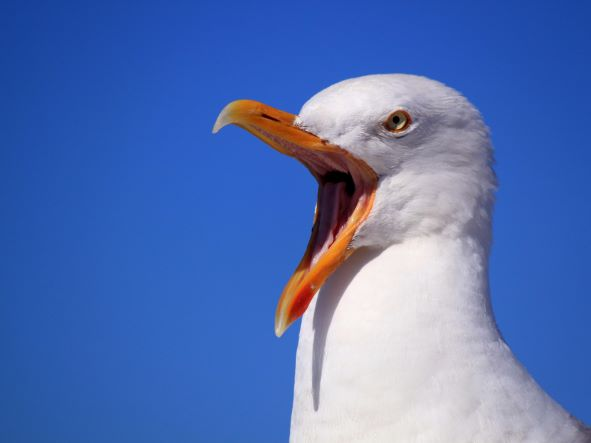
\includegraphics[width=.18\textwidth]{imgs/seagull/seagull.jpg}
  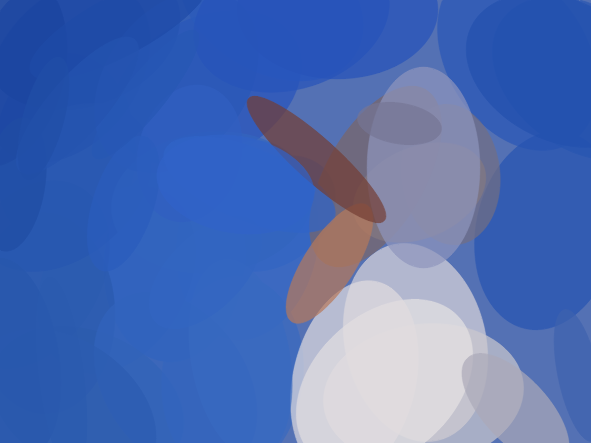
\includegraphics[width=.18\textwidth]{imgs/seagull/4.png}
  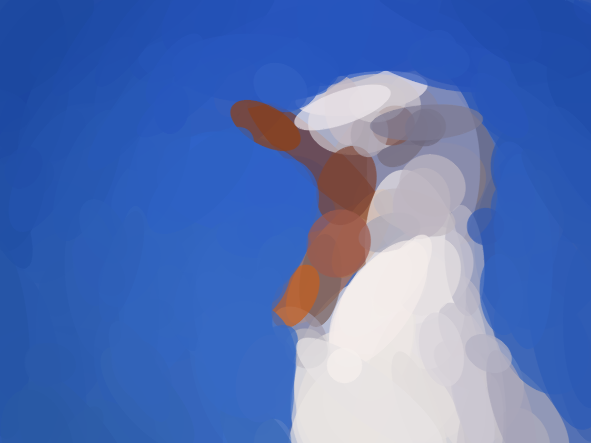
\includegraphics[width=.18\textwidth]{imgs/seagull/6.png}
  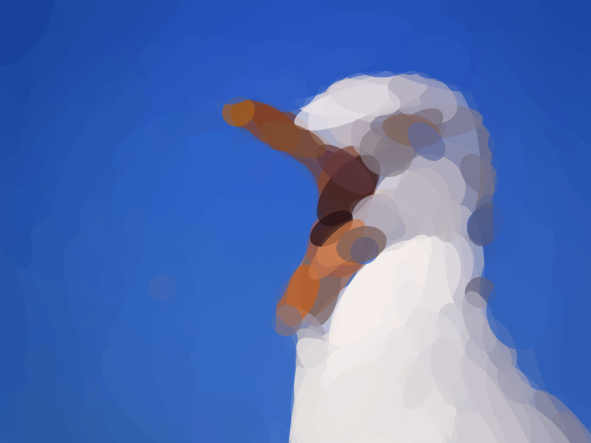
\includegraphics[width=.18\textwidth]{imgs/seagull/7.png}
  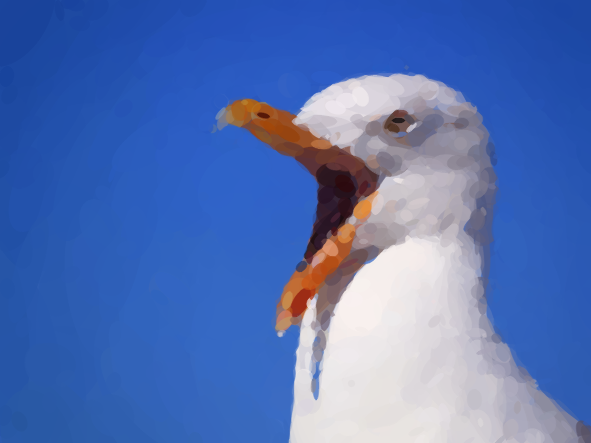
\includegraphics[width=.18\textwidth]{imgs/seagull/10.png}
  \caption{Seagull: The top line is the sampling mask at stage 200, 400, 600, 800, 1000. The bottom left image is the reference image, the other four images are the canvas at stage 50, 200, 600, 1000.}
  \label{fig:seagull}
\end{figure*}
\section{Related Work}

Roger Johansson is the first to use simple triangles to reproduce fine art\cite{evo-mona-lisa}. Although he claims to use the genetic programming method, he truly uses the hill climbing algorithm to optimize the colors, shapes, and positions of a group of triangles. In his algorithm, he optimize 50 triangles for about 1 million steps to get a similar result of the face of Mona Lisa. Because he optimizes all triangles as a whole, the method is hard to scale-up. Inspired by Roger Johansson, Michael Fogleman creates a macOS application \textit{Primitive} that can transfer an image into combination of geometric primitives \cite{primitive}. He uses the hill climbing algorithm and the simulated annealing algorithm to optimize the shape and position of each primitive one by one. Unlike Roger Johansson's algorithm, \textit{Primitive} doesn't optimize the color of each primitives, but samples the color from the reference image. Sam Twidale then creates another desktop application called \textit{Geometrize} that makes \textit{Primitive} cross-platform and easy to use\cite{geometrize}. Sebastian Proost uses a real genetic algorithm to optimize triangles to re-draw Van Gogh's The Starry Night\cite{starry-night}, but like Roger Johansson's work, he optimize 150 triangles as a whole, so the algorithm is not flexible enough and hard to scale up. Anastasia Opara implement the hill climbing algorithm as Roger Johansson\cite{genetic-drawing}, but she introduces a sampling mask to help the algorithm to focus on different area of the reference image in different stages.

\section{Algorithm Overview}

In this section I will first define the problem we want to solve, then introduce the basic algorithm and two main techniques of our algorithm to get better performance. 

To define the problem clearly, the input of the algorithm is a reference image(whether photographed or painted), we want the algorithm to output a series of semitransparent geometric primitives, by combining them one by one we can get a similar image as the reference. We call each of the semitransparent geometric primitives a "stroke". Also we want the algorithm to mimic the behavior of real human painting, i.e. first using large size stroke on the background, then small size stroke on the main body. To simplify the algorithm, we only consider the rotated ellipse as our strokes. Each stroke has 5 properties:
\begin{enumerate}
    \item color: $(r,g,b)$ 3 channels
    \item center position: $(x,y)$ on canvas
    \item size: $(sx,sy)$
    \item rotation angle: $r \in [0, 180)$
    \item opacity: $\alpha \in [0, 1]$
\end{enumerate}

The basic algorithm we use is genetic algorithms. In this problem, every stroke is a DNA, many strokes construct a population. The fitness of the DNA is evaluated as the similarity between the reference image and the canvas after drawing the stroke on. At every stage of the algorithm, we first initialize the population randomly, then evolve the population using cross over and mutation for some generations, at last draw the stroke with the most fitness on the canvas. However, directly applying this genetic algorithm does not work well as shown in Fig. \ref{fig:fail}. The shape and color of the stroke is a bit random, and all the details are last. To improve the result, we introduce two main techniques as follow.
\begin{figure}[htp]
  \centering
  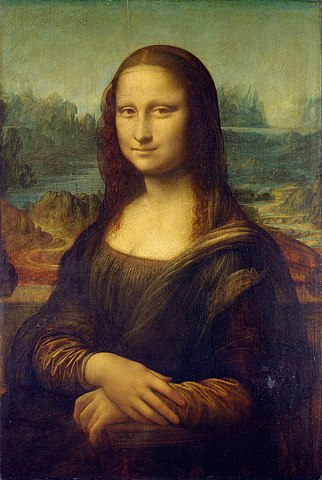
\includegraphics[width=.4\columnwidth]{imgs/monalisa-322px.jpg}
  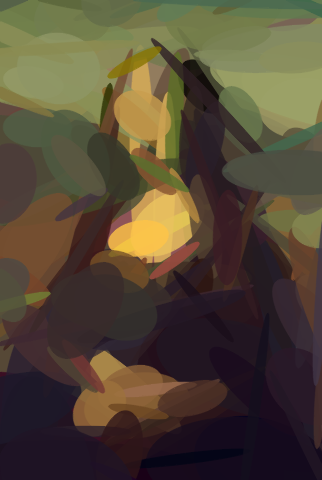
\includegraphics[width=.4\columnwidth]{imgs/failure-case.png}
  \caption{Failure case: the left is the reference image - the Mona Lisa by Leonardo da Vinci, the right is the result of the basic algorithm after 300 iterations.}
  \label{fig:fail}
\end{figure}
\paragraph{Space Reduction} Having so many parameters of one stroke, even we only optimize one stroke at one stage, the parameter space is still too large for the algorithm to find a global minimum. To solve this problem, one important observation is that we don't have to choose the globally best stroke at every step, because the stroke size is small compared with the canvas, there should have multiple plausible positions for one stroke. And even if we can't even find a plausible position, we can still paint the stroke on the canvas and hopefully it will be covered by other better strokes. As a result, we can randomly sample a small constraint area for the strokes at the beginning of each stage, and sample the population only inside the constraint area. And the same as \textit{primitive}\cite{primitive}, we can sample the color from the reference image, rather than optimize it from random. Further more, we can constrain the maximum and minimum size of the stroke at different stages, and fix the opacity at $0.7$. In this way we can largely reduce the searching space so the algorithm can easily find a good stroke. 

\paragraph{Sampling Mask} When human paints a picture, we usually first paint the background, then paint the main body. The background has less information and is more smooth, the main body has more information and has more edges. To let the algorithm mimic the behavior of human being, we create a series of sampling masks at different stages as shown in Fig. \ref{fig:seagull}. These masks are used to provide the position sampling probability in population initialization, and are created using the Gaussian blur of the gradient of the original image as in \cite{genetic-drawing}. At first the Gaussian kernel size is big so the algorithm has more chance to explore background on the canvas, then the kernel size is decreasing so the algorithm can focus on the foreground. With these masks the algorithm can complete the details on the main body rather than wasting on the background. 

\section{Implementation}

Alg. \ref{algo} shows the scheme of our algorithm, I'll introduce the details of each steps in this chapter.

\begin{algorithm}
    \caption{Genetic Painting}
    \begin{algorithmic}[1]
        \Require $I$ \Comment{Reference image}
        \Ensure $S$ \Comment{Painted image sequence}
        \State $canvas \gets \mathop{\mathrm{mean}}(I)$
        \State $S \gets [canvas]$
        \For{$s < stage\_max$}
            \State \Call{ComputeStrokeLimit}{$s$, $stage\_max$}
            \State \Call{CreateMask}{$I$, $s$, $stage\_max$}
            \State $P \gets \Call{InitPopulation}{I, pop\_size}$
            \State \Call{EvaluatePopulation}{$I$, $P$}
            \For{$g < generation\_max$}
                \State $Q \gets \Call{CrossOver}{P}$
                \State $Q \gets \Call{Mutation}{Q}$
                \State \Call{EvaluatePopulation}{$Q$}
                \State $P \gets \Call{BestPreservation}{P, Q}$
            \EndFor
            \State $p \gets argmin_{loss}(P)$
            \State $canvas \gets \Call{UpdateCanvas}{canvas, p}$
            \State $S \gets [S, canvas]$
        \EndFor
    \end{algorithmic}
    \label{algo}
\end{algorithm}

At first the canvas is cleared as the mean color of the reference image, then in each stage, the algorithm follows a traditional genetic algorithm routine. 

\paragraph{Initialization} For the stroke size limit, we set the maximum and minimum size at the beginning of the program and fix it at the first few stages, after some stages the maximum size and minimum size both begin to decease, and at the last few stages the size limit is fixed again. The limit at last stages affects the detailed level of the painted image, but the size limit at the beginning does not affect the final image that much. For the sampling masks we follow a similar idea. At first few stages the mask is all black meaning uniform distribution. Then the Gaussian blurred mask is computed and the Gaussian kernel size is decreasing from image size to one pixel. To compute the mask, we first transfer the reference image into gray scale, then compute the gradient in two directions, then change it into polar expression, then normalize the magnitude into $[0,1]$ and apply Gaussian blur. Apart from building masks from Gaussian blur, the difference between the canvas and the reference image is also used at the last stages helping the algorithm to finish the details on the main body. To initialize the population, we first randomly sample a point on the canvas using the sampling mask, and get the color of that point on the reference image. The stroke size is uniformly sampled between the size limit, the rotation is sampled based on the local gradient on that point as in \cite{genetic-drawing}:
\begin{equation}
    r = U(0, 180)\cdot (1-|\bm{d}|) + angle(\bm{d}) + 90
\end{equation}
This equation means: if the reference image has large gradient here, the stroke should better aligned with the edge, which is perpendicular to the gradient. But if the local gradient is small, the stroke can be drawn in random direction. By doing this, we get the first DNA in our population, and all the rest DNAs can be mutated from this DNA using the mutation operation introduced below.

\paragraph{Cross Over} The parents are sampled based on the fitness of each DNA. The fitness is computed as the negative of absolute difference $f$ between the reference image and the canvas after drawing the DNA on. We use dynamic linear regularization method for computing sampling probability:
\begin{equation}
    F_k = -f + f_{max} + \xi^k
\end{equation}
where $k$ is the generation number, $\xi=0.9$. After choosing two parents $p_1$ and $p_2$, we randomly let the child's position, size, and rotation angle from either $p_1$ or $p_2$ with equal probability. Continue this process until we get the next generation same size as the parent.

\paragraph{Mutation} We only mutate the position, size and rotation angle of the stroke. For the position, we let the stroke can move a little bit from the original point in two directions. For the stroke size, we let the stroke can shrink into half or extend double in either direction, and also need to satisfy the size limit. For the rotation angle, we just let the stroke to rotate freely. The three mutation operations have different possibilities depending on their influence on the result, for example we set the possibilities of them at $0.2$, $0.4$ and $0.4$.

\paragraph{Best Preservation} For better convergence rate, we preservation the best individual in the parent generation. We compare the best DNA in the parent generation and compare it with the best DNA in the child generation, if the parent generation performs better, we replace the worst DNA in the child generation with the parent's best, otherwise we do nothing.

\section{Results}

I implement the algorithm in C++ using the OpenCV library\cite{opencv_library}. The algorithm usually takes few minutes to converge on a regular image(around 500px). The differences between the canvas and the reference image at different stages are shown in Fig. \ref{fig:loss}, it shows our algorithm converges well.
\begin{figure}[htp]
  \centering
  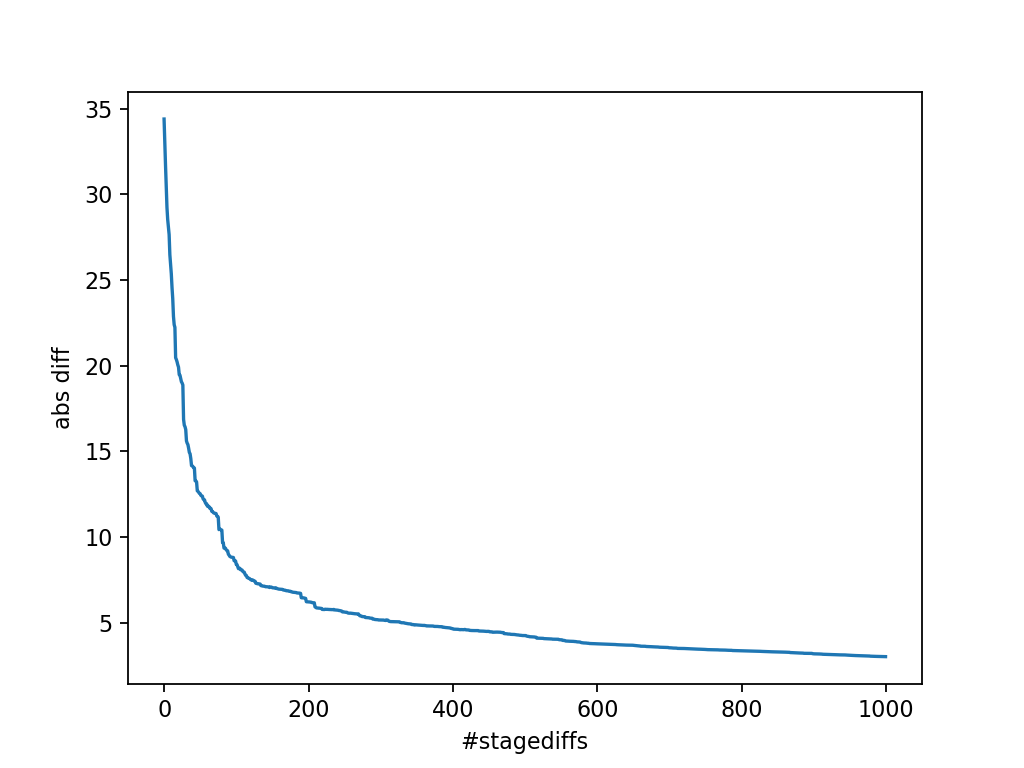
\includegraphics[width=\columnwidth]{imgs/seagull-loss.png}
  \caption{Difference Convergence}
  \label{fig:loss}
\end{figure}
The stages needed to get a good image largely depend on the complexity of the image. For example, in the seagull example(Fig. \ref{fig:seagull}) the algorithm can generate very detailed image like the reference in about 1000 stages, but in the Mona Lisa example(Fig. \ref{fig:monalisa}), the algorithm still needs more works on the face after 1000 stages. But we can see from the canvases in the early stages that the algorithm can approximate the reference image with very few strokes, this makes the algorithm able to generate stylized art works with simple geometries. 

\begin{figure*}[ht]
  \centering
  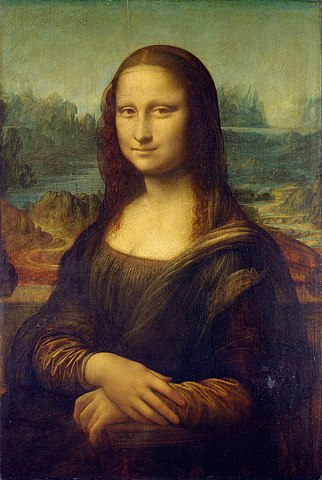
\includegraphics[width=.18\textwidth]{imgs/monalisa-322px.jpg}
  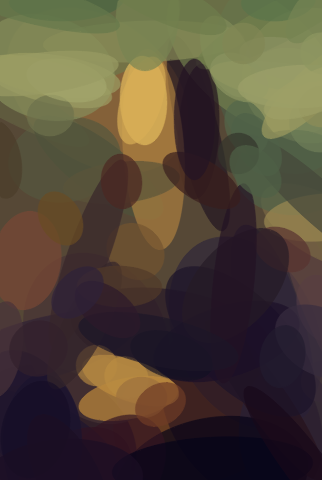
\includegraphics[width=.18\textwidth]{imgs/monalisa/stage100.png}
  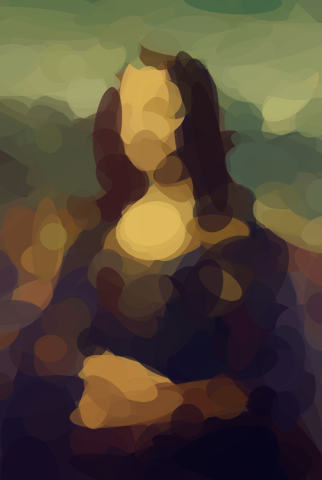
\includegraphics[width=.18\textwidth]{imgs/monalisa/stage300.png}
  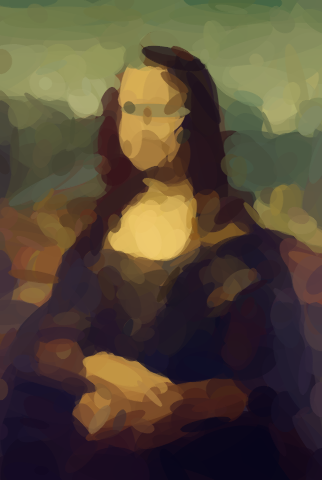
\includegraphics[width=.18\textwidth]{imgs/monalisa/stage600.png}
  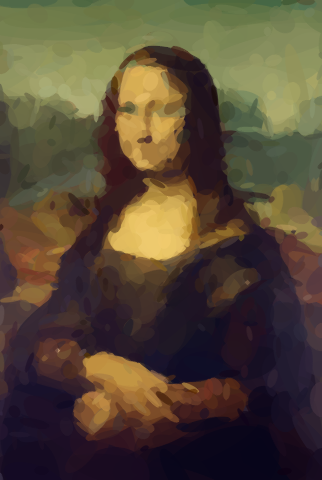
\includegraphics[width=.18\textwidth]{imgs/monalisa/stage999.png}
  \caption{Mona Lisa: The left most is the reference image, the rest images are the canvas at stage 100, 300, 600, 1000.}
  \label{fig:monalisa}
\end{figure*}

\begin{figure*}[ht]
  \centering
  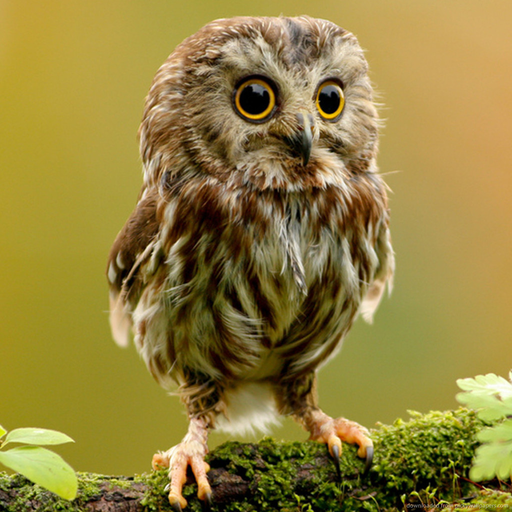
\includegraphics[width=.18\textwidth]{imgs/owl/owl.png}
  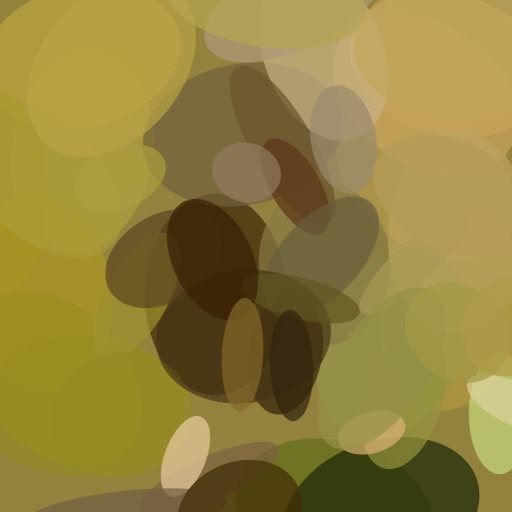
\includegraphics[width=.18\textwidth]{imgs/owl/stage50.png}
  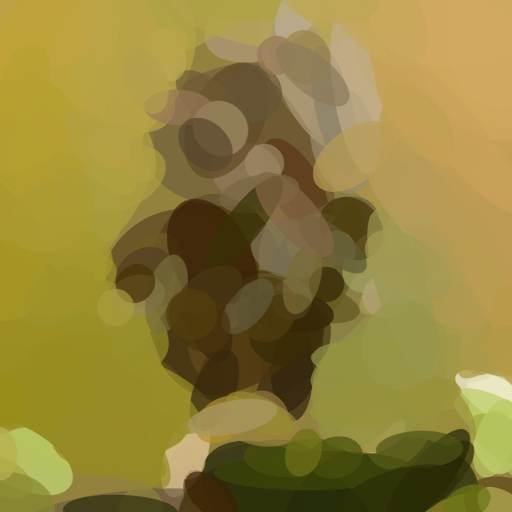
\includegraphics[width=.18\textwidth]{imgs/owl/stage200.png}
  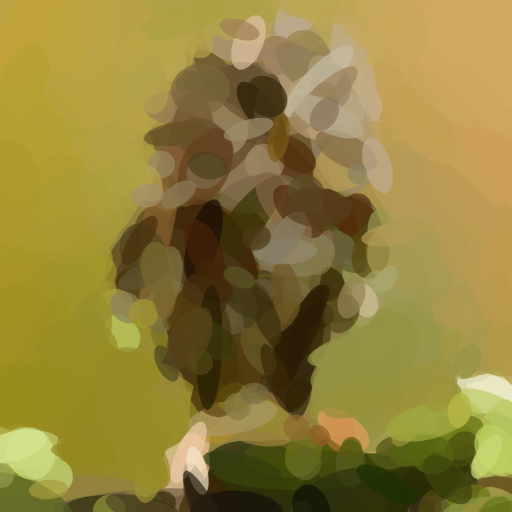
\includegraphics[width=.18\textwidth]{imgs/owl/stage400.png}
  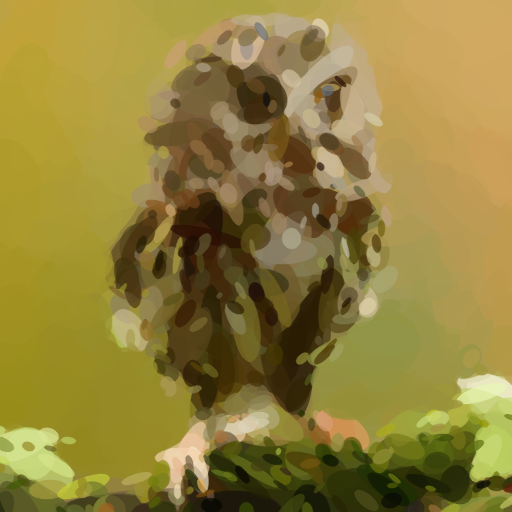
\includegraphics[width=.18\textwidth]{imgs/owl/stage800.png}
  \caption{Owl: The left most is the reference image, the rest images are the canvas at stage 50, 200, 400, 800.}
  \label{fig:owl}
\end{figure*}

\section{Limitation and Future Works}
Take a closer look at the face of Mona Lisa in Fig. \ref{fig:monalisa} and the eyes of the owl in Fig. \ref{fig:owl}, we can find the colors are preserved but the shape details are missing. When human paints a portrait, the painter usually spends a large portion of time on the face of the character. But for the computer, if the face only takes a small area on the canvas, the possibility of the algorithm to draw a stroke on the face is relatively small. To solve this problem one can try to use the face detection algorithm to create a sampling mask, force the algorithm to spend more time on the face of the main character.

Another drawback of this algorithm is efficiency, which can be improved by using parallel genetic algorithms\cite{10.1145/3400031}. At each stage this algorithm is a standard genetic algorithm, so it should be easily paralleled. At last the current implementation is not interactive enough, applications like \cite{primitive}\cite{geometrize} can adjust the shape and size at run time and have better GUI support. But this implementation is good enough to show the efficacy of the algorithm. 

\bibliographystyle{IEEEtran}
\bibliography{ref.bib}

\end{document}